\chapter{Testing the Algorithms} \label{testingChap}
\newcommand{\code}[1]{\lstinline|#1|}
\section{Overview}
While the algorithms of previous sections are of great theoretical interest,
questions remain on their practicality. To address this,
I have implemented the algorithms and tested their performance on
randomly generated instances of $ \arr $, simple stochastic games, and
shapley's stochastic games. The notable conclusions are roughly speaking as follows,
\begin{itemize}
  \item the most basic algorithms of value iteration, and simulating the $\arr$ walk outperform all of the
binary search stle algorithms in almost all cases in terms of query count and time,
\item \cref{fixDecompAlg} tends to be the most performant of the binary search style algorithms on the problems tested
  here,
  \item the fixpoint decomposition method described in \cref{fixDecompChapter} performs better than the asymptotically superior
monotone decomposition method described in \cref{monotoneDecompChap}.
\end{itemize}
\section{Method}
\subsection{Algorithm Implementation Detail}
\subsubsection{Implementation}
I implemented these algorithms in the progamming language C++. 
Complete source code can be found \href{https://github.com/angusjoshi/tarski}{here}
including all algorithms in \cref{stateAlgsChap},
and solvers for all problems in \cref{relatedProblemsChapter} using $\trsk$ algorithms.
Compilation and linking was done with
clang version 14.0.3 with the C++20 standard and \lstinline{-03} optimization settings.
Soplex\citep{soplex} was used as a dependency to solve linear programs
as part of the shapley's stochastic games solver.  \\
\subsubsection{Performance Improvements}
There are some performance optimizations that could be made. For simplicity of implementation\footnote{particularly
in implementing slices of functions as described in \cref{sliceDef}},
\lstinline{std::vector}s are shuffled and appended to unnecessarily, and I believe
performance could be gained by changing this. \lstinline{std::function} is the main abstraction for passing
the monotone functions around the system and are shown to be particularly innefficient in \citep{stdFunctionBad},
so I believe performance can be gained by changing this to something like the \lstinline{function_view}
described in \citep{stdFunctionBad}.
In performance profiling, I found \lstinline{soplex} was a bottleneck in solving shapley's stochastic games.
Perhaps \lstinline{soplex} is not optimized for solving a large number of very small LPs and a better alternative could be found.
There is also perhaps scope for using sensitivity
analysis as described in \citep{sensAnalysis} to reuse values from previous function queries to improve
solver performance; although this could be incredibly complex and not worth the effort.

\subsection{Random Problem Generation} \label{randomGen}
Instances of all three problems were generated randomly to facilitate testing. The method of randomization used
for each instance is detailed in this subsection. Throughout random numbers were generated using tools
from the \lstinline{<random>} header in the C++ standard library.
\subsubsection{\arr} \label{arrRandom}
Recall from \cref{arr} that an instance of the arrival problem consists of a directed graph with
a designated target vertex such that every vertex has exactly two labelled outgoing edges.
This leads to a natural notion of a random arrival instance on $n$ vertices $v_1, ..., v_n$.
Simply choose for each vertex $v_i$ the successors $s_0(v_i)$ and $s_1(v_i)$ uniformly at random
from the set of vertices, and note that it is without loss of generality to fix the target to be $v_n$.
Random instances for various fixed sizes of the $\arr$ problem were generated thusly for testing.

\subsubsection{Simple Stochastic Games} \label{ssgRandom}
Simple stochastic games do not have as natural a notion of random problem instances as $\arr$ for the following reasons,
\begin{itemize}
  \item vertices can be one of three types, 
  \item vertices can have different numbers of successors,
  \item chance vertices can have arbitrary probability distributions on their successors.
\end{itemize}
For simplicity, I generate a random simple stochastic game on $n$ vertices $v_1, ..., v_n$ as follows,
\begin{itemize}
  \item the type of each vertex is chosen uniformly at random from the three possibilities,
  \item all vertices have exactly two successors,
  \item the probability distribution on the two successors of a chance node is chosen by
    partitioning the interval $[0, 1]$ with a number chosen uniformly at random from the range $[0, 1]$.
  \item $v_n$ is fixed to be the target for the maximizer.
\end{itemize}

\subsubsection{Shapley's Stochastic Games} \label{shapleyRandom}
The degrees of freedom for defining an instance of shapley's stochastic games are as follows,
\begin{itemize}
  \item action sets can have arbitrary size at each state,
  \item for each joint action at each state, an arbitrary probability distribution on the all
    the states in the game can be chosen,
  \item payoffs for each joint action for each state can be chosen arbitrarily.
\end{itemize}
In order, these are addressed as follows,
\begin{itemize}
  \item both players have three actions at every state,
  \item payoff and successor matrices are all $3 \times 3$ (which follows from the above item),
  \item every entry in every successor matrix is a probability distribution on exactly two vertices.
    That is to say that at every state when a joint action is chosen the transition is chosen
    to be one of two states,
  \item every probability distribution in the successor matrix is chosen as a u.a.r. partition of $[0, 1]$
    as in the simple stochastic game case,
  \item all entries of the payoff matrices are chosen to be u.a.r. integers in the range $[-10, 10]$.
\end{itemize}
\subsubsection{Limitations}
I acknowledge that testing with random instances in this fashion is necessarily limited; the results
shown later give evidence that random generation in this fashion does not tend to generate 'hard' instances.
For instance, as will be shown in \cref{arrivalWalkPlot}, the length of the walk in a random instance
of the $\arr$ problem as described above seems to scale linearly with the size of the problem despite
the fact that in the worst case the walk can have an exponential length.
\subsection{Testing Protocol}
Separate tests were carried out for the three problems detailed in \cref{relatedProblemsChapter} as follows.
For all problems, all of the algorithms were tested with varying instance sizes. For simple stochastic games
and shapley's stochastic games all the algorithms were also tested with a fixed problem size and varying
approximation constant $\varepsilon$. In all tests, the number of queries to the monotone function is
measured, and the time to run the algorithm is measured. The measured time is precisely the time between
the function to run the algorithm is called, and the function returning with a fixpoint, so preprocessing
and other miscellaneous actions do not have an effect. All tests were repated 20 times with the
mean values recorded recorded. Different sizes were used for different algorithms in the same test
to ensure tests terminated in a reasonable amount of time. \\
The Kleene, Tarski \cref{kleeneTarski} was not tested directly on any of the monotone functions.
Instead, for shapley's and simple stochastic games, the continuous function is iterated on directly,
and for $\arr$ the walk is simulated directly. All of these are essentially the same as \cref{kleeneTarski}
but are slightly more performant due to skipping unnecessary scaling. \\
From here on I will denote the Fearnley, \pav, Savani algorithm described in \cref{fixDecompAlg}
as FPS, the Dang, Qi, and Ye algorithm descbribed in \cref{dQiYiAlg} as
DQY, Chen and Li described in \cref{monotoneDecompChap} as CL, and Kleene, Tarski 
described in \cref{kleeneTarski} as KT.
\subsubsection{\arr}
\begin{test}[Arrival Main] \label{arrMainTest}
  The three algorithms listed below were tested on random arrival instances as in \cref{arrRandom}
  with varying sizes between $3$ and $18$.
\end{test}
\begin{test}[Arrival Walk] \label{arrWalkTest}
  The arrival walk with preprocessing as in \cref{arrivalPreprocess} 
  was simulated to termination for random arrival instances with varying sizes
  between $10$ and $100000$.
\end{test}
\begin{test}[Long Arrival] \label{longArrivalTest}
  All algorithms were tested on the arrival instance with the
  longest possible walk, as seen in \cref{expLongArrival},
\end{test}
\subsubsection{Simple Stochastic Games}
\begin{test}[Simple Stochastic Game Main] \label{ssgMainTest}
  All algorithms were tested on random simple stochastic
  games as in \cref{ssgRandom} with varying sizes. The binary
  search algorithms were tested on sizes between $3$ and $13$.
  Value iteration was tested with sizes between $10$ and $100000$.
\end{test}
\begin{test}[Simple Stochastic Game Approximation] \label{ssgApproxTest}
  All four algorithms were tested on random simple stochastic
  games as in \cref{ssgRandom} with fixed size $N = 11$ and varying
  approximation constant $\varepsilon \in \{ 0.1, 0.01, 0.001, 0.0001, 0.00001, 0.000001 \}$.
\end{test}

\subsubsection{Shapley's Stochastic Games}
\begin{test}[Shapley Main] \label{shapleyMainTest}
  All algorithms were tested on random shapley's stochastic games
  as in \cref{shapleyRandom} with varying size. The binary search style algorithms
  were tested with sizes between $2$ and $6$. Value iteration was tested with
  sizes between $10$ and $40$.
\end{test}

\begin{test}[Shapley Approximation] \label{shapleyApproxTest}
  All algorithms were tested on random simple stochastic
  games as in \cref{shapleyRandom} with fixed size $N = 6$ and varying
  approximation constant $\varepsilon \in \{ 0.5, 0.1, 0.01, 0.001, 0.0001 \}$.
\end{test}

\section{Results} \label{resultsSec}
  \vspace{-15pt}
  \begin{figure}[H]
      \centering
      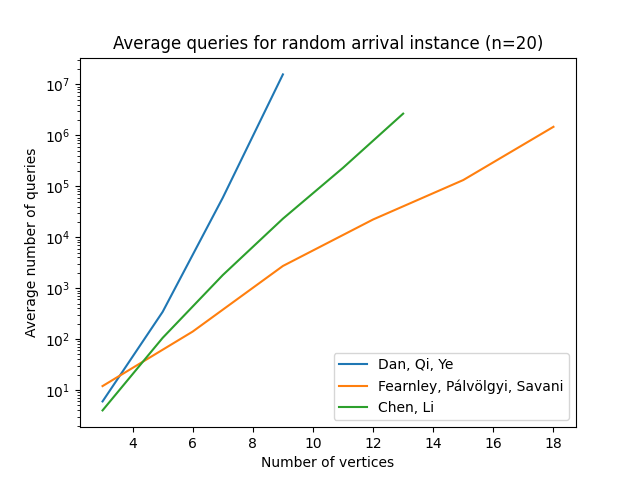
\includegraphics[width=2.6in]{plots/arrival_queries.png}
      \centering
      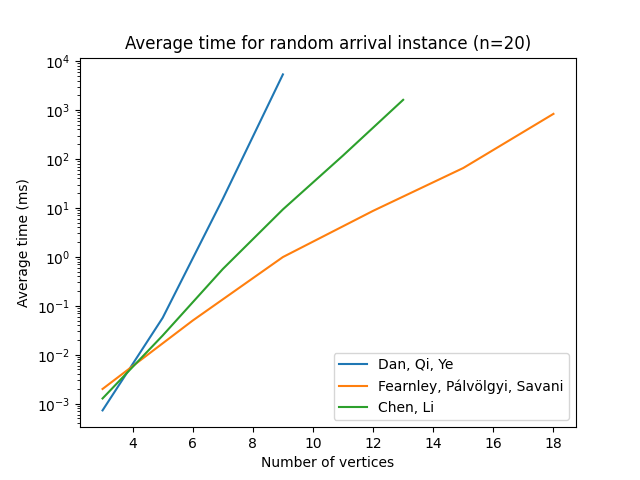
\includegraphics[width=2.6in]{plots/arrival_time.png}
      \caption{\cref{arrMainTest}} \label{arrivalMainPlot}
  \end{figure}
  \vspace{-22pt}
  \begin{figure}[H]
      \centering
      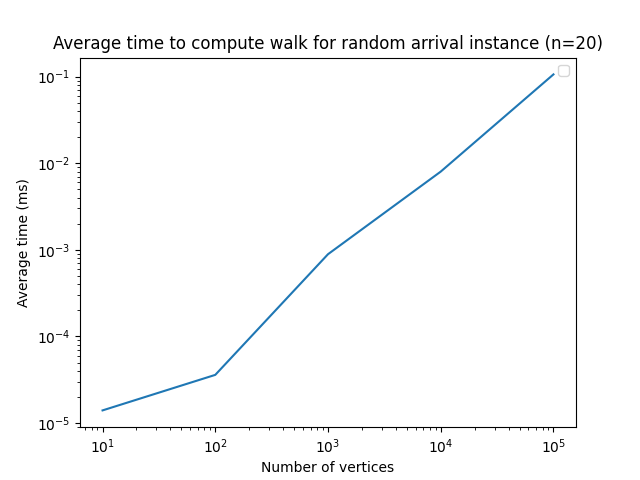
\includegraphics[width=2.6in]{plots/arrival_steps.png}
      \centering
      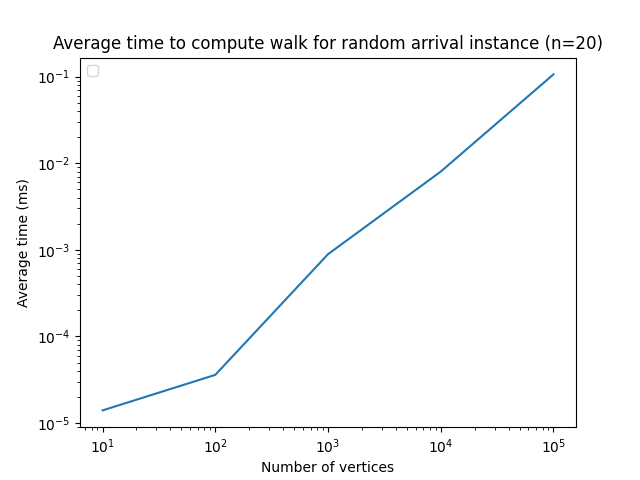
\includegraphics[width=2.6in]{plots/arrival_wtime.png}
      \caption{\cref{arrWalkTest}} \label{arrivalWalkPlot}
  \end{figure}
  \vspace{-22pt}
  \begin{figure}[H]
      \centering
      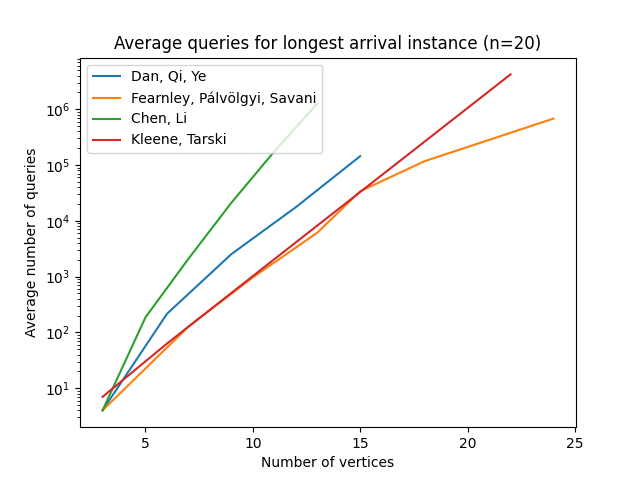
\includegraphics[width=2.6in]{plots/arrival_long_queries.png}
      \centering
      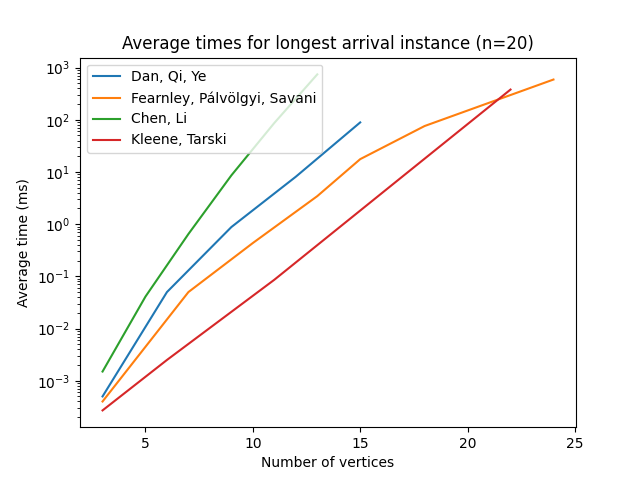
\includegraphics[width=2.6in]{plots/arrival_long_time.png}
      \caption{\cref{longArrivalTest}} \label{arrivalLongPlot}
  \end{figure}
  \vspace{-22pt}
  \begin{figure}[H] 
      \centering
      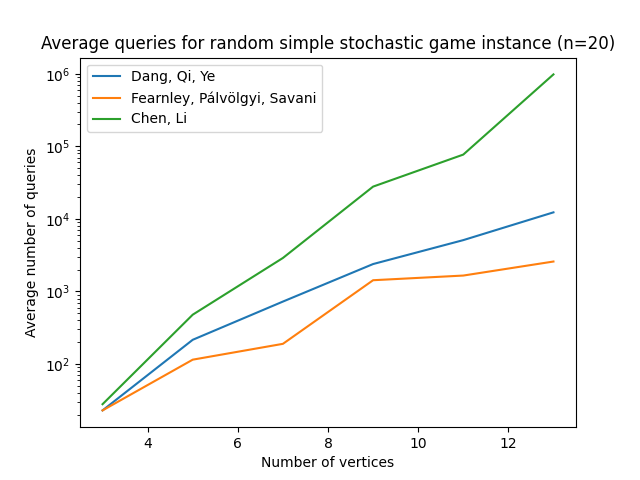
\includegraphics[width=2.6in]{plots/simple_queries.png}
      \centering
      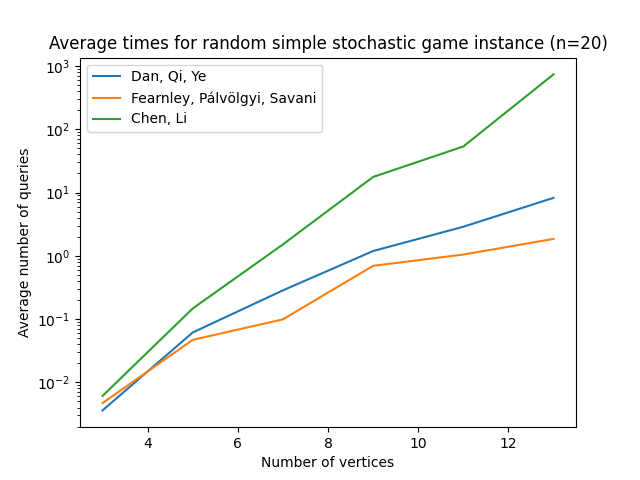
\includegraphics[width=2.6in]{plots/simple_time.png}
      \caption{\cref{ssgMainTest}} \label{simpleMainPlot}
  \end{figure}
  \vspace{-20pt}
  \begin{figure}[H]
      \centering
      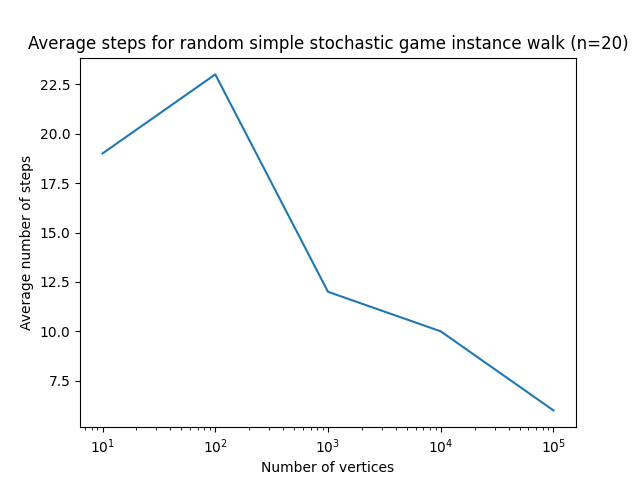
\includegraphics[width=2.6in]{plots/simple_steps.png}
      \centering
      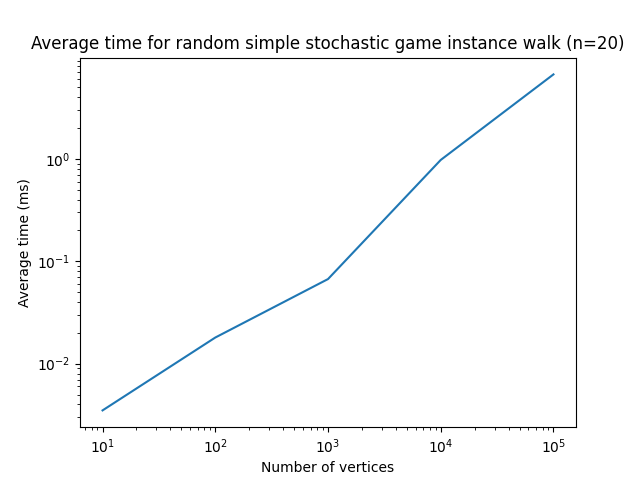
\includegraphics[width=2.6in]{plots/simple_wtime.png}
      \caption{\cref{ssgMainTest} cont.} \label{simpleWalkPlot}
  \end{figure}
  \vspace{-20pt}
  \begin{figure}[H]
      \centering
      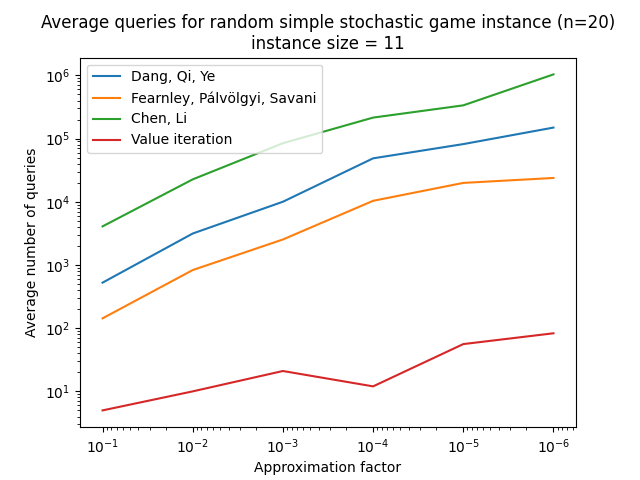
\includegraphics[width=2.6in]{plots/simple_eps_queries.png}
      \centering
      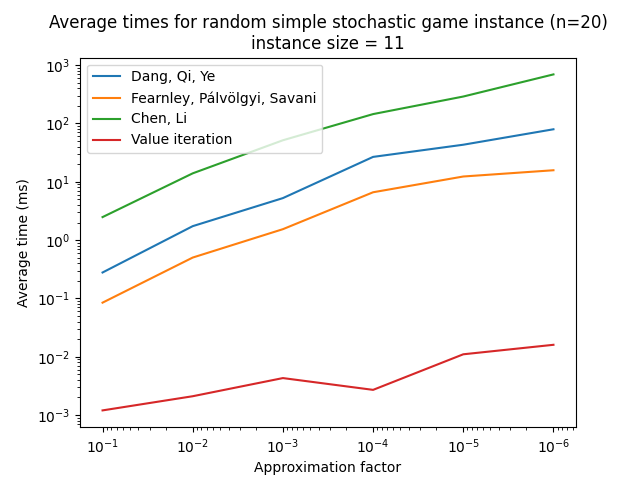
\includegraphics[width=2.6in]{plots/simple_eps_times.png}
      \caption{\cref{ssgApproxTest}} \label{simpleApproxPlot}
  \end{figure}
  \vspace{-20pt}
  \begin{figure}[H]
      \centering
      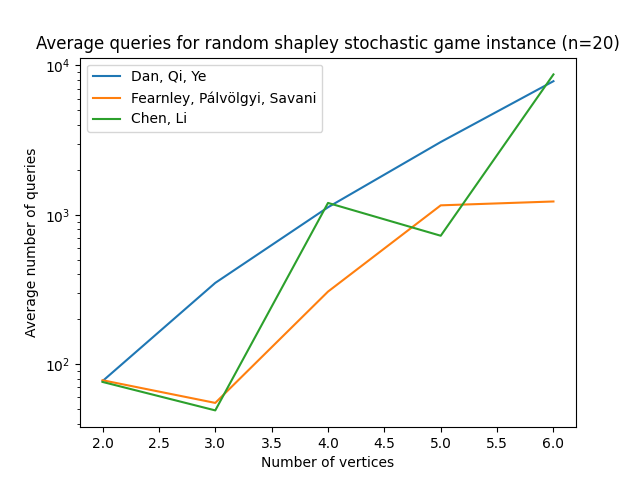
\includegraphics[width=2.6in]{plots/shapley_queries.png}
      \centering
      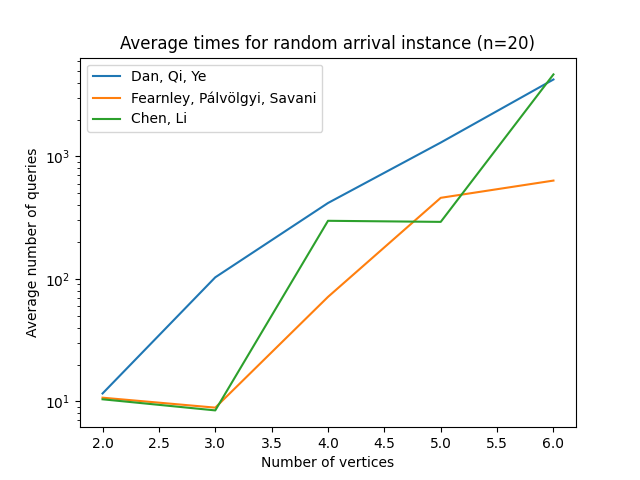
\includegraphics[width=2.6in]{plots/shapley_time.png}
      \caption{\cref{shapleyMainTest}} \label{shapleyMainPlot}
  \end{figure}
  \vspace{-20pt}
  \begin{figure}[H]
      \centering
      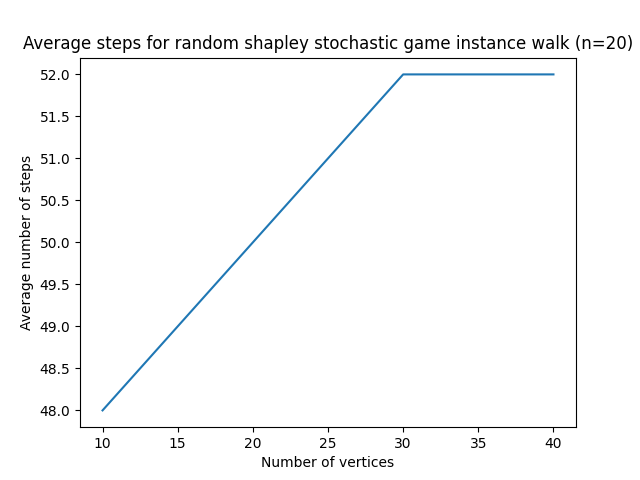
\includegraphics[width=2.6in]{plots/shapley_steps.png}
      \centering
      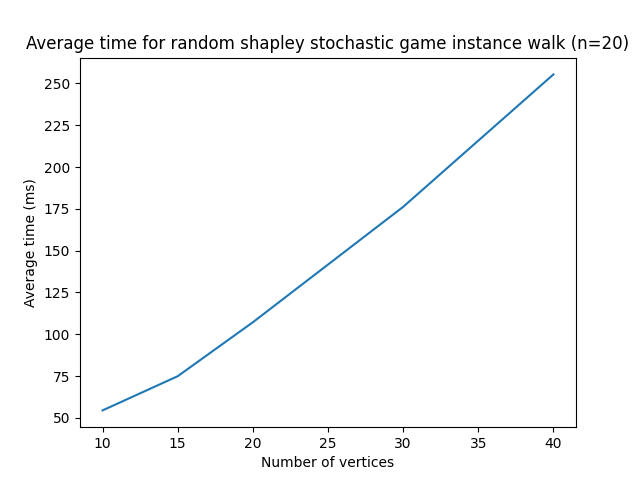
\includegraphics[width=2.6in]{plots/shapley_wtime.png}
      \caption{\cref{shapleyMainTest} cont.} \label{shapleyWalkPlot}
  \end{figure}
  \vspace{-20pt}
  \begin{figure}[H]
      \centering
      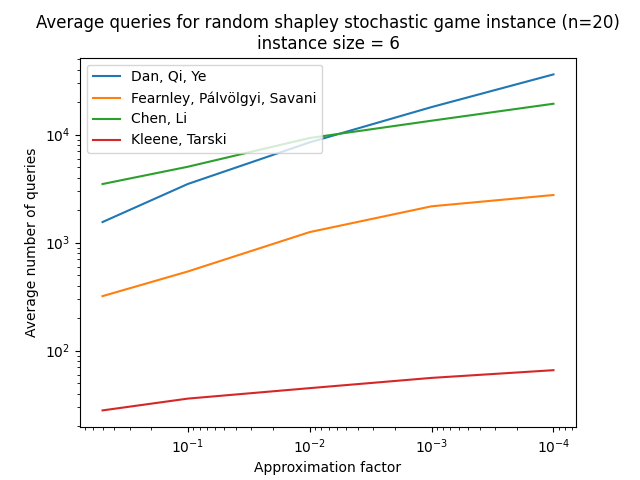
\includegraphics[width=2.6in]{plots/shapley_eps_queries.png}
      \centering
      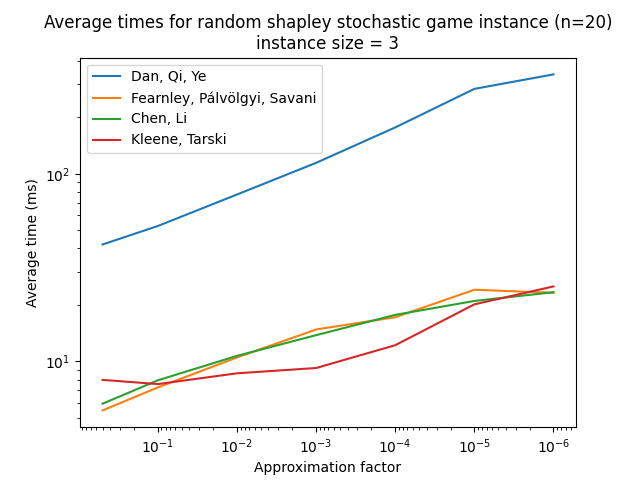
\includegraphics[width=2.6in]{plots/shapley_eps_times.png}
      \caption{\cref{shapleyApproxTest}} \label{shapleyApproxPlot}
  \end{figure}

%todo maybe add more to specific discussion sections relating
% asymptotic bounds
\section{Discussion}
On the whole, value iteration and simulating the $\arr$ walk tend to be
the most performant algorithms. Interestingly, FPS tends to be the most
performant of the binary search style algorithms, beating out the asymptotically
superior CL in almost all cases. More detailed discussion is given for individual cases below.
\subsection{$\arr$}
It can clearly be seen in \cref{arrivalMainPlot} and \cref{arrivalWalkPlot}
that simulating the arrival walk vastly outperforms the binary-search based
algorithms on randomly generated instances of the arrival problem.
The distinction is less clear when testing with the worst case instance
for the walk as seen in \cref{arrivalLongPlot}; FPS outperforms the walk
in terms of query count for more than 15 vertices, and in terms of time for more than
20. This is somewhat unexpected as the number of steps in the walk on
the worst case instance is $\Theta(2^n)$, while the upper bound we
get from FPS when applied to the walk is 
$O(\log^{\lceil (n + 2)/3 \rceil } (2^n)) = O(n^{\lceil (n + 2)/3 \rceil})$,
which is clearly a weaker bound than $O(2^n)$. I believe the cause of this
is that the recursive binary search algorithms work particularly well
on this specific long walk instance; the fixpoint for this specific instance
will be something like $\vec{x} = (2^{n}, 2^{n - 1}, ..., 1)$, and the
binary search algorithms always start by querying midpoints which happen
to be powers of two so coincide exactly with the actual fixpoint.
This perhaps motivates further testing- are there other instances
for which FPS outperforms the walk?  \\
In comparing the binary search style algorithms, it can be seen that
FPS performs best in all cases, and in particular performs better
than the asymptotically superior CL algorithm. The difference between
CL and DQY is less clear however; for random instances CL performs
better as seen in \cref{arrivalMainPlot},
but DQY performs better on the long walk instance as seen in \cref{arrivalLongPlot}.

\subsection{Simple Stochastic Games}
Similarly to $\arr$, value iteration is the most performant algorithm for solving
random simple stochastic games - it even seems to be the case
that the number of queries goes \emph{down} as the number of vertices
goes up for the walk as seen in \cref{simpleWalkPlot}. 
I believe that this is a limitation of the method
of random instance generation which perhaps motivates further investigation
into methods for generating 'hard' simple stochastic games. It could also
be the case that testing with a fixed approximiation factor $\varepsilon$
and stopping probability $\beta$ causes this behaviour. \\
In comparing the binary search based algorithms, it can be seen in \cref{simpleMainPlot} 
that
FPS is again the most performant, and DQY is the least performant. The difference
between FPS and CL is small in this case however. \\
In the test with varying approximation factor as seen in \cref{simpleApproxPlot}, value iteration 
is again the most performant, with FPS the best of the binary search algorithms.
DQY is again the slowest, with CL in the middle. Varying the approximation factor
for the simple stochastic game problem has the effect of changing the height of the lattice
that is searched; if $\beta$ is the stopping probability, and $\varepsilon$ is the approximation
factor, the associated discretized function is 
defined on $\left[\left \lfloor \frac{1}{\beta \varepsilon}\right \rfloor\right]^d$.
Since KT runs in worst case complexity $O(Nd)$ where $N$ is the height of the lattice,
and FPS in $O(\log^{\lceil \frac{2n + 2}{3} \rceil} N)$, one might expect that for
very small approximation factors that FPS is more performant. This is not shown in
the results however, so perhaps more investigation should be done into finding
instances of simple stochastic games which are 'hard' for value iteration.

\subsection{Shapley's Stochastic Games}
Testing on shapley's stochastic games was much more limited than the other two problems
as the associated monotone function took a lot longer to compute. It could be the case
the the LP solver that I used (\lstinline{soplex}\citep{soplex}) is not optimized for solving
many thousands of small LPs, or that solving LPs in this fashion will necessarily
take significantly more time than the functions for $\arr$ and simple stochastic games. \\
In comparing the algorithms running on random instances, it can be seen in \cref{shapleyMainPlot}
and \cref{shapleyWalkPlot} that 
again value iteration is the most performant. DQY is the least performant on random instances, and the difference
between CL and FPS is small. Interestingly, there seems to be some association between
the parity of the dimension and the performance of CL and FPS. I believe this is because of the
$\lceil \cdot \rceil$ in the exponent of their complexities caused by
subproblems with dimension less than 3 during decomposition, and the only reason
we don't see this in other plots is because we are measuring with less granularity on size.
Perhaps this motivates testing with more datapoints on the other problems as well. \\
The test with varying approximation factor as seen in \cref{shapleyApproxPlot} shows
again that value iteration is the most performant, and FPS is the most performant of the binary search algorithms.
There is not much difference between CL and DQY in this case. Similarly to simple stochastic games,
one would expect that for very small approximation factors that the binary search algorithms
perform better than value iteration - but again this is not seen in the results for these tests. This is again
perhaps motivation for more investigation in finding 'hard' stochastic games for the value iteration algorithm. \\
In shapley's stochastic games, many parameters were also unchanged through all tests. The maximum value
in the payoff matrix for shapley's could be varied, the stopping probabilities for both,
the number of actions at each state in shapley's, and the number of successors for all states in both
problems could all be varied. 


\section{Further Work}
The main shortcoming of the testing I have carried out is the random instance generation described in \cref{randomGen}.
In all problems, the results such as \cref{arrivalWalkPlot} give strong evidence
that for the most basic algorithms like simulating the walk and value iteration,
my scheme for random problem generation does not generate 'hard' problems so investigation
into this could be carried out. Another extension
could be to implement strategy improvement and quadratic programming
to solve simple stochastic games and further compare.\\
In \citep{valueIterationTest} both of these issues are somewhat addressed when testing value iteration,
strategy improvement, and quadratic programming on simple stochatic games. The authors
build a library of extremal problems that are difficult for particular algorithms, as well as a more
sophisticated method of generating random problems than I have done here. Perhaps transitive
comparisons can be made to results in \citep{valueIterationTest} given
we have both tested value iteration, although the difference in how we generate problems makes this tenuous. \\
Time could be spent on on optimizing the monotone function for shapley's stochastic games,
as tests have been limited to small sizes so an increase in performance could yield more interesting data. \\
The asymptotic advantage the binary-search style algorithms achieve over the iterative algorithms
is dependent on the ratio between the height of the lattice and it's dimension. In particular
the asymptotic bound for FPS is stronger than KT if $d \in o(\frac{\log N}{\log \log N})$.
In simple and shapley's stochastic games, solving to higher precision $\varepsilon$ causes
an increase in the height of the searched lattice so testing with very high precision
approximation constraints along with finding 'hard' instances of these problems could
demonstrate a practical advantage to FPS over value iteration. This would require additional support
in my implementation for high precision numerical types such as GMP\citep{gmp}, and
I believe finding an LP solver for shapley's stochastic games 
with strong support for high precision types will also be difficult.
%todo note on strategy improvement

